\chapter[%
    Linear-Response Density Cumulant Theory for Excited States:\\
	First Implementation and Benchmark Calculations
]{%
    Linear-Response Density Cumulant Theory for Excited States:\\
	First Implementation and Benchmark Calculations\footnote{%
        A.~V.~Copan and A.~Yu.~Sokolov (to be submitted in
        J.~Chem.~Theory~Comput).
    }
}
\label{ch:response}


\section{Abstract}

We present a linear-response formulation of density cumulant functional theory
(DCT) that provides accurate access to many electronic states.
DCT expresses the electronic energy as a Hermitian, size-extensive, and
stationary functional of the one-particle density matrix and the two-particle
density cumulant.
In the original DCT formulation only the information about a single electronic
state (usually, the ground state) is obtained.
In this research, we combine DCT with linear response theory to obtain
information about many electronic states simultaneously.
We discuss the derivation of linear-response DCT, present its implementation for
the ODC-12 method (LR-ODC-12), and benchmark its performance against highly
accurate equation-of-motion coupled cluster theory with up to full triple
excitations (EOM-CCSDT).
Our results for a set of small molecules demonstrate that LR-ODC-12 vertical
excitation energies are in closer agreement with EOM-CCSDT than those obtained
from equation-of-motion coupled cluster theory with up to double excitations
(EOM-CCSD).
In addition, we report a linear-response formulation of the orbital-optimized
linearized coupled cluster theory with double excitations (LR-OLCCD), which we
obtain by neglecting the non-linear terms in the LR-ODC-12 equations.


\section{Introduction}

Accurate simulation of excited electronic states remains one of the major
challenges in modern electronic structure theory. 
{\it Ab initio}\/ methods for excited states can be divided into
single-reference and multi-reference categories, based on their ability to
treat static electron correlation.
Multi-reference methods can correctly describe static correlation in
near-degenerate valence orbitals and electronic states with multiple-excitation
character, but often lack accurate treatment of important dynamic correlation
effects (e.g., multi-configurational self-consistent field or multi-reference
perturbation theories)
\cite{Knowles:1985p259,Werner:1985p5053,Wolinski:1987p225,Hirao:1992p374,Finley:1998p299,Andersson:1990p5483,Andersson:1992p1218,Werner:1996p645,Angeli:2001p10252,Angeli:2001p297}
or become very costly when the number of near-degenerate orbitals is large
(e.g., multi-reference configuration interaction or coupled cluster theories).
\cite{Mukherjee:1977p955,Lindgren:1978p33,Siegbahn:1980p1647,Jeziorski:1981p1668,Werner:1988p5803,Mahapatra:1998p157,Mahapatra:1999p6171,Pittner:2003p10876,Evangelista:2007p024102,Datta:2011p214116,Evangelista:2011p114102,Kohn:2013p176,Nooijen:2014p081102}
Meanwhile,
single-reference methods
\cite{Foresman:1992p135,Sherrill:1999p143,Geertsen:1989p57,Comeau:1993p414,Stanton:1993p7029,Krylov:2008p433,Crawford:2000p33,Shavitt:2009,Sekino:1984p255,Koch:1990p3345,Koch:1990p3333,Nooijen:1997p6441,Nooijen:1997p6812,Nakatsuji:1978p2053,Nakatsuji:1979p329}
often provide a compromise between the computational
cost and accuracy, and can be used to reliably compute properties of molecules
in low-lying electronic states near the equilibrium geometries. In these
situations, single-reference equation-of-motion coupled cluster theory
(EOM-CC)
\cite{Geertsen:1989p57,Comeau:1993p414,Stanton:1993p7029,Krylov:2008p433,Crawford:2000p33,Shavitt:2009}
is usually the method of choice, especially when high accuracy
is desired. 

The EOM-CC methods yield size-intensive excitation energies
\cite{Koch:1990p3345,Koch:1990p3333}
and can be
systematically improved by increasing the excitation rank of the cluster
operator in the exponential parametrization of the wavefunction. Although EOM-CC
is usually formulated in the context of a similarity-transformed Hamiltonian,
its excitation energies are equivalent to those obtained from linear-response
coupled cluster theory (LR-CC).
\cite{Sekino:1984p255,Koch:1990p3345,Koch:1990p3333}
Both EOM-CC and LR-CC are based on non-Hermitian eigenvalue problems,
complicating the computation of molecular properties (e.g., transition dipoles)
by requiring evaluation of left and right eigenvectors.
\cite{Stanton:1993p8840,Stanton:1994p4695,Stanton:1994p8938,Levchenko:2005p224106}
Several Hermitian alternatives to EOM-CC and LR-CC have been
proposed to avoid these problems, such as  
algebraic diagrammatic construction
\cite{Schirmer:1982p2395,Schirmer:1991p4647,Schirmer:2004p11449,Harbach:2014p064113,Dreuw:2014p82}, 
unitary and variational LR-CC,
\cite{Taube:2006p3393,Kats:2011p062503,Walz:2012p052519}
similarity-constrained CC,
\cite{Kjonstad:2017p4801}
and propagator-based LR-CC.
\cite{Moszynski:2005p1109,Korona:2010p14977}

In this work, we present the development of linear-response density cumulant
functional theory (LR-DCT), a size-intensive approach for excited
electronic states. In density cumulant functional theory (DCT),
\cite{Kutzelnigg:2006p171101,Simmonett:2010p174122,Sokolov:2012p054105,Sokolov:2013p024107,Sokolov:2013p204110,Sokolov:2014p074111,Wang:2016p4833}
the
electronic energy is obtained by optimizing the energy functional directly in
terms of the one-particle reduced density matrix and the two-particle density
cumulant, a fully connected part of the two-particle reduced density matrix
(2-RDM).
\cite{Fulde:1991,Ziesche:1992p597,Kutzelnigg:1997p432,Mazziotti:1998p419,Mazziotti:1998p4219,Kutzelnigg:1999p2800,Ziesche:2000p33,Herbert:2007p261,Kong:2011p214109,Hanauer:2012p50}
In this regard, DCT is related to approaches that are based on
the variational optimization
\cite{Colmenero:1993p979,Nakatsuji:1996p1039,Mazziotti:1998p4219,Mazziotti:2006p143002,Kollmar:2006p084108,DePrince:2007p042501,DePrince:2016p164109}
or parametrization
\cite{Mazziotti:2008p253002,Mazziotti:2010p062515,DePrince:2012p1917}
of 2-RDM\@. On
the other hand, DCT has a close relationship
\cite{Sokolov:2013p024107,Sokolov:2013p204110}
with wavefunction-based electronic
structure theories, such as linearized, unitary, and variational coupled
cluster theory.
\cite{Kutzelnigg:1991p349,Kutzelnigg:1998p65,VanVoorhis:2000p8873,Kutzelnigg:1982p3081,Bartlett:1989p133,Watts:1989p359,Szalay:1995p281,Cooper:2010p234102,Evangelista:2011p224102}
In contrast to variational 2-RDM theory
\cite{Nakata:2009p042109,vanAggelen:2010p114112,Verstichel:2010p114113}
and traditional
coupled cluster methods [e.g., CCSD and CCSD(T)],
\cite{Crawford:2000p33,Shavitt:2009}
DCT naturally combines
size-extensivity and a Hermitian energy functional. In addition, the DCT
electronic energy is fully relaxed with respect to all of its parameters, which
greatly simplifies computation of the first-order molecular properties.
\cite{Scheiner:1987p5361,Salter:1989p1752,Gauss:1991p2623,Gauss:1991p207}
We have successfully applied DCT to a variety of chemical systems with
different electronic structure effects (e.g., open-shell, symmetry-breaking,
and multi-reference).
\cite{Sokolov:2013p204110,Sokolov:2014p074111,Wang:2016p4833,Copan:2014p2389,Mullinax:2015p2487}
One limitation of the original DCT formulation is
that it can only obtain information about the lowest-energy state of a
particular symmetry (usually, the ground state). By combining DCT with linear
response theory, we remove this limitation, providing access to many electronic
states simultaneously.

We begin with a brief overview of linear response theory (\cref{sec:lr}).
We then discuss the derivation of linear-response theory for the ODC-12 method
(LR-ODC-12, \cref{sec:lr_odc12}).
In section \cref{sec:olccd}, 
we derive equations for the linear-response orbital-optimized linearized
coupled cluster theory with double excitations (LR-OLCCD), which we obtain by
neglecting the non-linear terms in the LR-ODC-12 equations. 
We outline the
computational details in \cref{sec:comp_details}.
In section \cref{sec:results}, we demonstrate that the LR-ODC-12 excitation
energies are size-intensive (\cref{sec:size_intensivity}), test the performance
of LR-ODC-12 for the dissociation of \ce{H2} (\cref{sec:two_electron}), and
benchmark the accuracy of LR-ODC-12 for vertical
excitation energies of small molecules (\cref{sec:vert_excit}).
% Finally, we present our conclusions in section \cref{sec:conclusions}.


\section{Theory}

\subsection{Linear Response Theory}
\label{sec:lr}
We now briefly review linear response theory in the quasi-energy
formulation.\cite{Norman:2011p20519}
The quasi-energy of a system perturbed by a time-dependent interaction
\(\hat{V}f(t)\) is defined as
\begin{equation}
    Q(t)
    =
    \langle\Psi(t)|
    \hat{H} + \hat{V} f(t) - i\tfrac{\partial}{\partial t}
    |\Psi(t)\rangle
\end{equation}
where \(\Psi(t)\) is the phase-isolated wavefunction, from which the usual
Schr\"odinger wavefunction can be recovered as
\(
    e^{-i\int_0^t dt' Q(t')}
    \Psi(t)
\).
Assuming that the perturbation is periodic
\begin{equation}
    f(t)
    =
    \sum_\omega f(\omega) e^{-i\omega t}
\end{equation}
the time average of the quasi-energy over a period of oscillation, denoted as 
\(
    \{Q(t)\}
\),
is variational with respect to the exact dynamic state.\cite{Helgaker:2012p543}
The independent parameters \(\mathbf{u}(t)\) that define such a state can be
written using a Fourier expansion
\begin{equation}
    \label{eq:parameter-fourier-expansion}
    \mathbf{u}(t)
    =
    \sum_{n=0}^\infty
    \sum_{\omega_1\cdots \omega_n}
    \mathbf{u}(\omega_1,\ldots, \omega_n)
    e^{-i(\omega_1+\cdots+\omega_n)t}
\end{equation}
where the outer sum runs over polynomial orders in \(f(t)\).
The stationarity of the time-averaged quasi-energy then implies the following
relationship\cite{Kristensen:2009p044112}
\begin{equation}
    \label{eq:linear-response-equation}
    \begin{array}{l}
        0
        =
        \left.
            \dfrac{d}{df(\omega)}
            \dfrac{%
                \partial \{Q(t)\}
            }{%
                \partial \mathbf{u}^\dagger(\omega)
            }
        \right|_{f=0}
        =
        \\[20pt]
        \left.
            \dfrac{%
                \partial^2 \{Q(t)\}
            }{%
                \partial \mathbf{u}^\dagger(\omega)
                \partial \mathbf{u}(\omega)
            }
            \dfrac{\partial \mathbf{u}(\omega)}{\partial f(\omega)}
        \right|_{f=0}
            +
        \left.
            \dfrac{%
                \partial^2 \{Q(t)\}
            }{%
                \partial \mathbf{u}^\dagger(\omega)
                \partial f(\omega)
            }
        \right|_{f=0}
    \end{array}
\end{equation}
which constitutes a linear equation for the first-order response of the system
to the perturbation. 
When the frequency $\omega$ is in resonance with an excitation energy of the
system, \cref{eq:linear-response-equation} will result in an infinite
first-order response
\(
    \dfrac{\partial \mathbf{u}(\omega)}{\partial f(\omega)}
\).
From \cref{eq:linear-response-equation}, we find that these poles occur when the
Hessian matrix of the quasi-energy with respect to the wavefunction parameters
\(\mathbf{u}(\omega)\) becomes singular.
We can express this Hessian matrix in the form
\begin{equation}
    \label{eq:quasi-energy-hessian}
    \left.
        \frac{\partial^2\{Q(t)\}}{%
            \partial \mathbf{u}^\dagger(\omega)
            \partial \mathbf{u}(\omega)
        }
    \right|_{f=0}
    \equiv
    \mathbf{E}
    -
    \omega\,
    \mathbf{M}
\end{equation}
where \(\mathbf{E}\) is the Hessian of the time-averaged electronic energy
\(\{\langle\Psi(t)|\hat{H}|\Psi(t)\rangle\}\) and \(\omega\mathbf{M}\) is the
Hessian of the time-derivative overlap
\(\{\langle\Psi(t)|i\dot{\Psi}(t)\rangle\}\).
The excitation energies of the system $\omega_k$ can therefore be determined by
solving the following generalized eigenvalue equation:
\begin{equation}
    \label{eq:linear-response-energy-eigenvalue-equation}
    \mathbf{E}\mathbf{z}_k
    =
    \omega_k
    \mathbf{M}\mathbf{z}_k
\end{equation}
where \(\mathbf{M}\) serves as the metric matrix.
\Cref{eq:linear-response-energy-eigenvalue-equation} allows the determination of
excitation energies for an arbitrary parametrization of $|\Psi(t)\rangle$.

The generalized eigenvectors \(\mathbf{z}_k\) can be used to
compute transition properties for excited states.
In particular, in the exact linear response theory\cite{Olsen:1985p3235} the transition strength
of the perturbing interaction,
\(
    |\langle\Psi|\hat{V}|\Psi_k\rangle|^2
\),
is equal to the complex residue of the following quantity at
\(\omega\rightarrow\omega_k\):
\begin{equation}
    \langle\!\langle \hat{V}; \hat{V} \rangle\!\rangle_\omega
    \equiv
    \left.
    \mathbf{v}'^\dagger
    \cdot
    \frac{\partial \mathbf{u}(\omega)}{\partial f(\omega)}
    \right|_{f=0}
\end{equation}
This quantity is known as the linear response function and
\(
    \mathbf{v}'
\)
is termed the property gradient vector,\cite{Sauer:2011} which is defined as
follows:
\begin{equation}
    \label{eq:property-gradient-vector}
    \mathbf{v}'
    \equiv
    \left.
    \frac{%
        \partial^2 \{Q(t)\}
    }{%
        \partial \mathbf{u}^\dagger(\omega)
        \partial f(\omega)
    }
    \right|_{f=0}
\end{equation}
Substituting \cref{eq:property-gradient-vector,eq:quasi-energy-hessian} into
\cref{eq:linear-response-equation} and decomposing the quasi-energy Hessian as
\begin{equation}
    \mathbf{E} - \omega\mathbf{M}
    =
    (\mathbf{Z}^\dagger)^{-1}
    (\mathbf{Z}^\dagger \mathbf{M} \mathbf{Z})
    (\boldsymbol\Omega - \omega\mathbf{1})
    (\mathbf{Z})^{-1}
\end{equation}
where \(\boldsymbol\Omega\) is a diagonal matrix of generalized eigenvalues and
\(\mathbf{Z}\) is a matrix of generalized eigenvectors that simulataneously
diagonalizes \(\mathbf{E}\) and \(\mathbf{M}\), we obtain the
general formula for the transition strengths:
\begin{equation}
    \lim_{\omega\rightarrow \omega_k}
    (\omega-\omega_k)
    \langle\!\langle \hat{V}; \hat{V} \rangle\!\rangle_\omega
    =
    \frac{%
        |\mathbf{z}_k^\dagger \mathbf{v}'|^2
    }{%
        \mathbf{z}_k^\dagger \mathbf{M}\mathbf{z}_k
    }
\end{equation}
In \cref{sec:lr_odc12}, we will use the quasi-energy formalism to derive
equations for the linear-response ODC-12 method (LR-ODC-12).


\subsection{Linear-Response ODC-12}
\label{sec:lr_odc12}
In the ODC-12 method, the electronic energy Hessian can be written in the following
form
\begin{equation}
    \label{eq:lr-odc12-hessian-blocks}
    \mathbf{E}
    =
    \begin{pmatrix}
        \mathbf{A}_{11} & \mathbf{A}_{12} & \mathbf{B}_{11} & \mathbf{B}_{12} \\
        \mathbf{A}_{21} & \mathbf{A}_{22} & \mathbf{B}_{21} & \mathbf{B}_{22} \\
        \mathbf{B}_{11}^* & \mathbf{B}_{12}^* & \mathbf{A}_{11}^* & \mathbf{A}_{12}^* \\
        \mathbf{B}_{21}^* & \mathbf{B}_{22}^* & \mathbf{A}_{21}^* & \mathbf{A}_{22}^* \\
    \end{pmatrix}
\end{equation}
where the submatrices are defined in general as
\begin{equation}
    \label{eq:hessian-blocks}
    \mathbf{A}_{nm}
    =
    \left.
    \frac{\partial^2 E}{%
        \partial \mathbf{t}_n^\dagger
        \partial \mathbf{t}_m
    }
    \right|_{f=0}
    ,\ 
    \mathbf{B}_{nm}
    =
    \left.
    \frac{\partial^2 E}{%
        \partial \mathbf{t}_n^\dagger
        \partial \mathbf{t}_m^*
    }
    \right|_{f=0}.
\end{equation}
These complex derivatives relate to the second derivatives of the
electronic energy with respect to variations of the orbitals ($\mathbf{A}_{11}$, $\mathbf{B}_{11}$) and
cumulant parameters ($\mathbf{A}_{22}$, $\mathbf{B}_{22}$).
Similarly, the mixed second derivatives couple variations in the orbitals
and cumulant parameters ($\mathbf{A}_{12}$, $\mathbf{B}_{12}$). 
The metric matrix \(\mathbf{M}\) has a block-diagonal structure, as a
consequence of the linear parametrization of the wavefunction in
\cref{eq:odc12-wavefunction}:
\begin{equation}
    \label{eq:lr-odc12-metric-blocks}
    \mathbf{M}
    =
    \begin{pmatrix}
        \mathbf{S}_{11} & \mathbf{0} & \mathbf{0} & \mathbf{0} \\
        \mathbf{0} & \mathbf{1}_2 & \mathbf{0} & \mathbf{0} \\
        \mathbf{0} & \mathbf{0} & -\mathbf{S}_{11}^* & \mathbf{0} \\
        \mathbf{0} & \mathbf{0} & \mathbf{0} & -\mathbf{1}_2 \\
    \end{pmatrix}
\end{equation}
where
\(
    \mathbf{1}_2
    =
    \langle\Phi|\mathbf{a}_2^\dagger \mathbf{a}_2|\Phi\rangle
\)
is an identity matrix over the space of unique two-body excitations and the
orbital metric is defined as follows:
\begin{equation}
    \label{eq:metric-blocks}
    \omega\mathbf{S}_{11}
    =
    \left.
        \frac{\partial^2 \{\langle\Psi(t)|i\dot\Psi(t)\rangle\}}{%
            \partial \mathbf{t}_1^\dagger(\omega)
            \partial \mathbf{t}_1(\omega)
        }
    \right|_{f=0}
\end{equation}
Equations for all blocks of $\mathbf{E}$, $\mathbf{M}$, and the property
gradient vector $\mathbf{v}'$ are shown explicitly in the Supporting
Information (\cref{sec:suppinfo}).
We note that, due to the Hermitian nature of the DCT energy functional
\eqref{eq:energy-expression}, the ODC-12 energy Hessian $\mathbf{E}$ is always
symmetric.
As a result, in the absence of instabilities (i.e., as long as the Hessian is
positive semi-definite), the LR-ODC-12 excitation energies are guaranteed to
have real values.

To illustrate the derivation of the LR-ODC-12 energy Hessian, let us consider
the diagonal two-body block of \(\mathbf{E}\).
Expressing the energy \eqref{eq:energy-expression} using the cumulant expansion
\eqref{eq:two-body-n-rep} and differentiating with respect to $\mathbf{t}_2$, we
obtain:
\begin{equation}
    \label{eq:odc12-hessian-initial-form}
    \begin{array}{r@{\,}l}
        \mathbf{A}_{22}
        =
        \dfrac{\partial^2 E}{%
            \partial\mathbf{t}_2^\dagger
            \partial\mathbf{t}_2
        }
        =
        &
        f_p^q
        \dfrac{\partial^2 \gamma^p_q}{%
            \partial\mathbf{t}_2^\dagger
            \partial\mathbf{t}_2
        }
        +
        \overline{g}_{pr}^{qs}
        \dfrac{\partial \gamma^p_q}{\partial\mathbf{t}_2^\dagger}
        \dfrac{\partial \gamma^r_s}{\partial\mathbf{t}_2}
        \\[15pt]
        &
        +
        \tfrac{1}{4}
        \overline{g}_{pq}^{rs}
        \dfrac{\partial^2 \lambda^{pq}_{rs}}{%
            \partial\mathbf{t}_2^\dagger
            \partial\mathbf{t}_2
        }
    \end{array}
\end{equation}
where we have introduced the generalized Fock matrix
\(
    f_p^q
    \equiv
    h_p^q
    +
    \overline{g}_{pr}^{qs}
    \gamma^r_s
\).
The derivatives of the one-body density matrix can be expressed in terms of the derivatives of the density cumulant
\begin{equation}
    \begin{array}{r@{\,}l}
    \label{eq:a22_odc12}
	\mathbf{A}_{22}
        =
        &
        \mathcal{F}_p^q
        \dfrac{\partial^2 \lambda^{pt}_{qt}}{%
            \partial\mathbf{t}_2^\dagger
            \partial\mathbf{t}_2
        }
        +
        \mathcal{G}_{pr}^{qs}
        \dfrac{\partial \lambda^{pt}_{qt}}{\partial\mathbf{t}_2^\dagger}
        \dfrac{\partial \lambda^{ru}_{su}}{\partial\mathbf{t}_2}
        \\[15pt]
        &
        +
        \tfrac{1}{4}
        \overline{g}_{pq}^{rs}
        \dfrac{\partial^2 \lambda^{pq}_{rs}}{%
            \partial\mathbf{t}_2^\dagger
            \partial\mathbf{t}_2
        }
    \end{array}
\end{equation}
where the intermediates $\mathcal{F}_p^q$ and $\mathcal{G}_{pr}^{qs}$ can be computed using a transformation of the one- and two-electron integrals to the natural spin-orbital basis (see \cref{sec:appendix} for details).
These cumulant derivatives are straightforward to evaluate from \cref{eq:odc12-wavefunction,eq:cumulant-parametrization} using either algebraic or diagrammatic techniques.

Next, let us outline the derivation of the one-body metric.
Substituting \cref{eq:odc12-wavefunction} into \cref{eq:metric-blocks} gives
\begin{equation}
    \label{eq:odc12-s11-metric}
    \begin{array}{r@{\,}l}
        \omega
        \mathbf{S}_{11}
        =
        &
        \left.
            \dfrac{1}{2}
            \dfrac{%
                \partial^2
                \{\langle\Psi|
                    [i\dot{T}_1^\dagger(t), T_1(t)]
                |\Psi\rangle\}
            }{%
                \partial \mathbf{t}_1^\dagger(\omega)
                \partial \mathbf{t}_1(\omega)
            }
        \right|_{f=0}
        \\[20pt]
        &
        -
        \left.
            \dfrac{1}{2}
            \dfrac{%
                \partial^2
                \{\langle\Psi|[T_1^\dagger(t), i\dot{T}_1(t)]|\Psi\rangle\}
            }{%
                \partial \mathbf{t}_1^\dagger(\omega)
                \partial \mathbf{t}_1(\omega)
            }
        \right|_{f=0}
    \end{array}
\end{equation}
where we have assumed that we are working in the variational orbital basis so that
\(
    T_1(t)|_{f=0}
    =
    0
\),
and
\(
    \Psi
    =
    \Psi(t)|_{f=0}
\)
denotes the ground state wavefunction.
Using the Fourier expansion of the $\mathbf{t}_1(t)$ parameters
(\cref{eq:parameter-fourier-expansion}), the gradients of the time derivatives
can be evaluated as:
\begin{equation}
    \label{eq:time_deriv_1}
    \left.
    \frac{%
        \partial i \dot{T}_1^\dagger(t)
    }{%
        \partial \mathbf{t}_1^\dagger(\omega)
    }
    \right|_{f=0}
    =
    -
    \omega
    \mathbf{a}_1^\dagger
    e^{+i\omega t}
\end{equation}
\begin{equation}
    \label{eq:time_deriv_2}
    \left.
    \frac{%
        \partial i \dot{T}_1(t)
    }{%
        \partial \mathbf{t}_1(\omega)
    }
    \right|_{f=0}
    =
    +
    \omega
    \mathbf{a}_1
    e^{-i\omega t}
\end{equation}
Substituting \cref{eq:time_deriv_1,eq:time_deriv_2} into \cref{eq:odc12-s11-metric} and evaluating the gradients
of \(T_1\) and \(T_1^\dagger\) similarly gives the final working equation for
the one-body metric:
\begin{equation}
    \begin{array}{r@{\,}l}
        \omega
        (\mathbf{S}_{11})_{ia,jb}
        &=
        \omega
        \langle\Psi|
        [a_a^i, a_j^b]
        |\Psi\rangle
        \\[10pt]
        &=
        \omega
        (
            \delta^b_a
            \gamma^i_j
            -
            \delta^i_j
            \gamma^b_a
        )
    \end{array}
\end{equation}


\subsection{Linear-Response OLCCD}
\label{sec:olccd}
The orbital-optimized linearized coupled cluster doubles method (OLCCD) can be considered as an approximation to the ODC-12 method where all of the non-linear $\mathbf{t}_2$ terms are neglected. Similarly, we can formulate the linear-response OLCCD method (LR-OLCCD) by linearizing the LR-ODC-12 equations. This simplifies the expressions for the electronic Hessian blocks that involve the second derivatives with respect to $\mathbf{t}_2$. For example, for the $\mathbf{A}_{22}$ block, we obtain:
\begin{equation}
    \label{eq:a22_olccd}
    \mathbf{A}_{22}
    =
    (f_0)_i^j
    \dfrac{\partial^2 \lambda^{ir}_{jr}}{%
        \partial\mathbf{t}_2^\dagger
        \partial\mathbf{t}_2
    }
    -
    (f_0)_a^b
    \dfrac{\partial^2 \lambda^{ar}_{br}}{%
        \partial\mathbf{t}_2^\dagger
        \partial\mathbf{t}_2
    }
    +
    \tfrac{1}{4}
    \overline{g}_{pq}^{rs}
    \dfrac{\partial^2 \lambda^{pq}_{rs}}{%
        \partial\mathbf{t}_2^\dagger
        \partial\mathbf{t}_2
    }
\end{equation}
where
\(
    (f_0)_p^q
    =
    h_p^q
    +
    \overline{g}_{pi}^{qi}
\)
is the usual (mean-field) Fock operator.
Comparing \cref{eq:a22_olccd} with \cref{eq:a22_odc12} from the LR-ODC-12
method, we observe that the former equation can be obtained from the latter by
replacing the $\mathcal{F}_p^q$ intermediates with the mean-field Fock matrix
elements and ignoring the term that depends on $\mathcal{G}_{pr}^{qs}$.
These simplifications arise from the fact that the $\mathcal{F}_p^q$ and
$\mathcal{G}_{pr}^{qs}$ intermediates contain high-order $\mathbf{t}_2$
contributions that are not included in the linearized LR-OLCCD formulation (see
\cref{sec:appendix} and Ref.\@ \citenum{Sokolov:2013p024107} for details).
For the $\mathbf{B}_{22}$ block, we find that all of the Hessian elements are
zero.
A complete set of working equations for LR-OLCCD is given in the Supporting
Information (\cref{sec:suppinfo}).


\section{Computational Details}
\label{sec:comp_details}
The LR-ODC-12 and LR-OLCCD methods were implemented as a standalone Python
program, which was interfaced with \textsc{Psi4}\cite{Parrish:2017p3185} and
\textsc{Pyscf}\cite{Sun:2018pe1340} to obtain the one- and two-electron
integrals.
Our implementation of the energy Hessian was validated by computing the static
response function for a dipole perturbation (i.e., the dipole polarizability):
\begin{equation}
    \langle\!\langle\hat{V}; \hat{V}\rangle\!\rangle_0
    =
    -
    \mathbf{v}'^\dagger
    \mathbf{E}^{-1}
    \mathbf{v}'
\end{equation}
This quantity can be evaluated numerically as a derivative of the ground state
energy
\begin{equation}
    \langle\!\langle\hat{V}; \hat{V}\rangle\!\rangle_0
    =
    \left.
    \frac{%
        d^2 E
    }{%
        df^2
    }
    \right|_{f=0}
\end{equation}
by perturbing the one-electron integrals
\(
    h_p^q
    \leftarrow
    h_p^q
    +
    f
    v_p^q
\)
with the integrals of the perturbing dipole operator, \(v_p^q\), and solving the
ODC-12 or OLCCD equations for different values of \(f\).
In this way, we have matched our response calculation to \(10^{-9}\ \au\) for
the electric dipole polarizability along the \(C_2\) symmetry axis of water.


We used \textsc{Q-Chem} 4.4\cite{QChem} to obtain results from
equation-of-motion coupled cluster theory with single and double excitations
(EOM-CCSD) and EOM-CCSD with triple excitations in the EOM part [EOM-CC(2,3)].
The \textsc{MRCC} program\cite{MRCC} was used to obtain results for
equation-of-motion coupled cluster theory with up to full triple excitations
(EOM-CCSDT).
All electrons were correlated in all computations.
We used tight convergence parameters in all ground-state ($10^{-8}$ \hartree)
and excited-state computations ($10^{-5}$ \hartree).
In \cref{sec:two_electron,sec:vert_excit}, the augmented aug-cc-pVTZ and
d-aug-cc-pVTZ basis sets of Dunning and co-workers were
employed.\cite{Kendall:1992p6796}
To compute vertical excitation energies in \cref{sec:vert_excit}, geometries of
molecules were optimized using ODC-12 (for LR-ODC-12), OLCCD (for LR-OLCCD), or
CCSD [for EOM-CCSD, EOM-CC(2,3), and EOM-CCSDT].

\section{Results and Discussion}
\label{sec:results}

\subsection{Size-Intensivity of the LR-ODC-12 Energies}
\label{sec:size_intensivity}

\begin{table*}[h!]
    \centering
    \caption{%
        \label{tab:size_int}
        Ground-state energies (in \hartree) and vertical excitation energies (in
        eV) for the four lowest-energy excited states of the CO molecule and
        noninteracting systems of CO with Ne atoms (\mbox{CO $+$ $n$Ne}, $n$ =
        1, 2, 3) computed using the ODC-12 and LR-ODC-12 methods (cc-pVDZ basis
        set).
        The noninteracting systems were separated from each other by \mbox{10000
        \AA} and the C--O bond distance was set to 1.12547 \AA\@.
        Results demonstrate size-intensivity of the LR-ODC-12 excitation
        energies.
    }
    \begin{tabular}{ccccc}
        \hline
        \hline
        & CO & CO $+$ Ne & CO $+$ 2Ne & CO $+$ 3Ne \\
        \hline
        \({X}\,^1\Sigma_g^+\) & $-$113.051282 & $-$241.730913 & $-$370.410543 & $-$499.090174\\
        \({}^3\Pi\) & 6.48596 & 6.48596 & 6.48596 & 6.48596 \\
        \({}^3\Sigma^+\) & 8.41225 & 8.41225 & 8.41225 & 8.41225 \\
        \({}^1\Pi\) & 8.90866 & 8.90866 & 8.90866 & 8.90866 \\
        \({}^3\Delta\) & 9.33189 & 9.33189 & 9.33189 & 9.33189 \\
        \hline
        \hline
    \end{tabular}
\end{table*}

All DCT methods are by construction {\it size-extensive}, meaning that their electronic energies scale linearly with the number of electrons.
In this section, we demonstrate that the LR-ODC-12 excitation energies are {\it
size-intensive}, i.e.\@ they satisfy the following property: $E(A^*+B) = E(A^*)
+ E(B)$, where $A$ and $B$ are two noninteracting fragments in their
corresponding ground states and $A^*$ is the fragment $A$ in an excited state.
\Cref{tab:size_int} shows the ODC-12 ground-state energies and the LR-ODC-12
excitation energies for the CO molecule and noninteracting systems composed of
CO and the neon atoms separated by 10000 \AA\ (\mbox{CO $+$ $n$Ne}, $n$ = 1, 2,
3).
The scaling of the ODC-12 energies for the ground \({X}\,^1\Sigma_g^+\)
electronic state is perfectly linear up to $10^{-8}$ \hartree, which is the
convergence parameter used in our ODC-12 computations.
Upon the addition of the neon atoms, the excitation energies of the CO molecule
remain constant up to the convergence threshold set in LR-ODC-12 ($10^{-6}$
eV).
These results provide numerical evidence that the LR-ODC-12 excitation energies
are size-intensive.


\subsection{H$_2$ Dissociation}
\label{sec:two_electron}

\begin{figure*}[h!]
    \centering
    \subfloat[]{\label{fig:H2_diss_odc}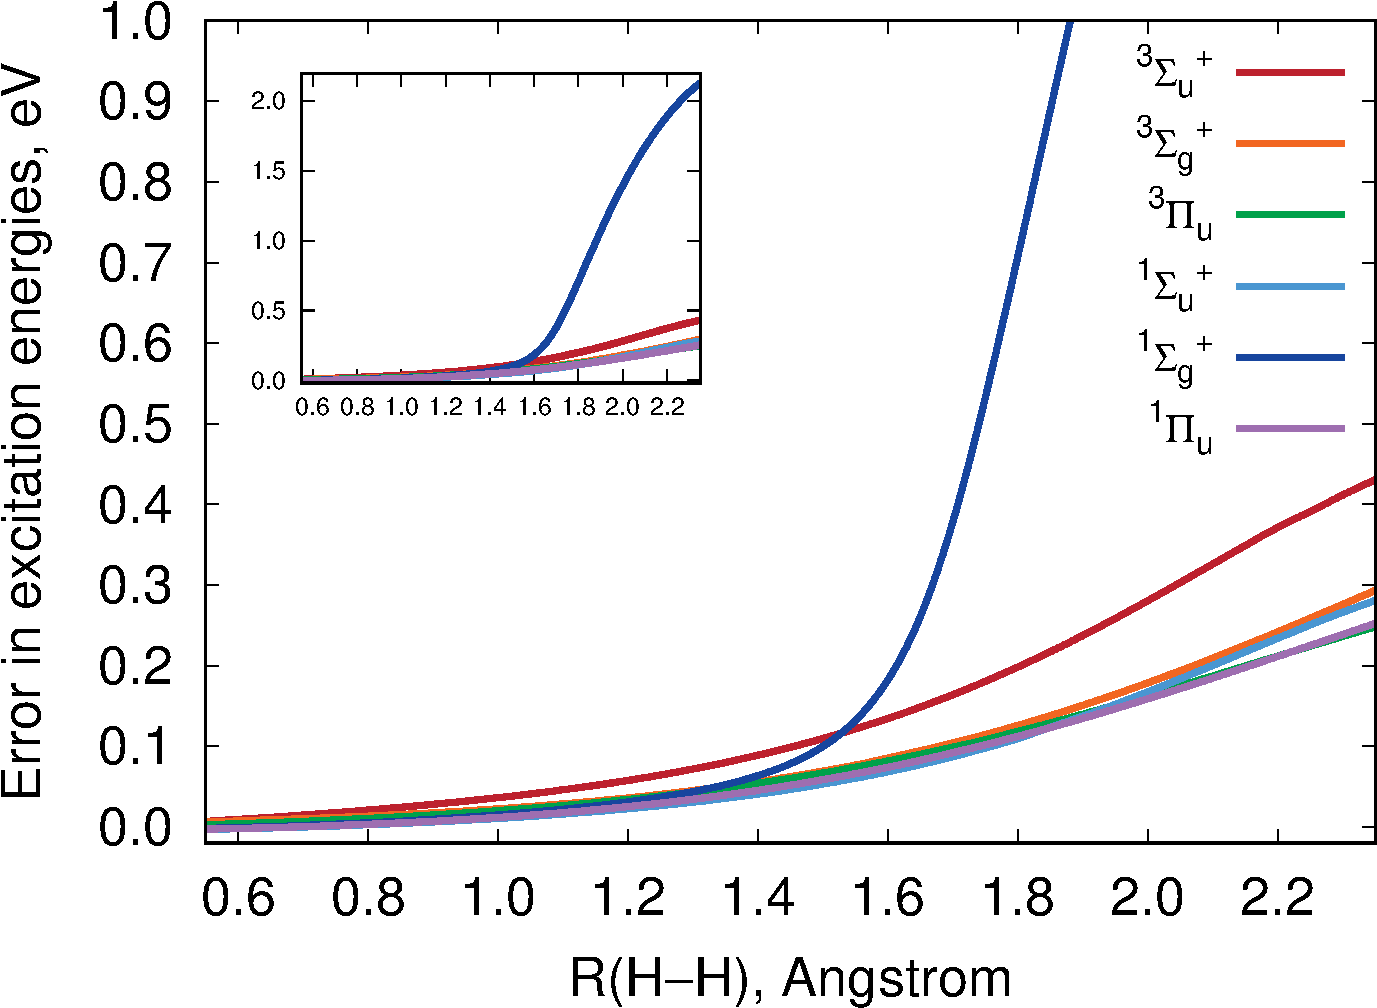
\includegraphics[width=0.45\textwidth]{figures/H2_odc.pdf}} \qquad
    \subfloat[]{\label{fig:H2_diss_olccd}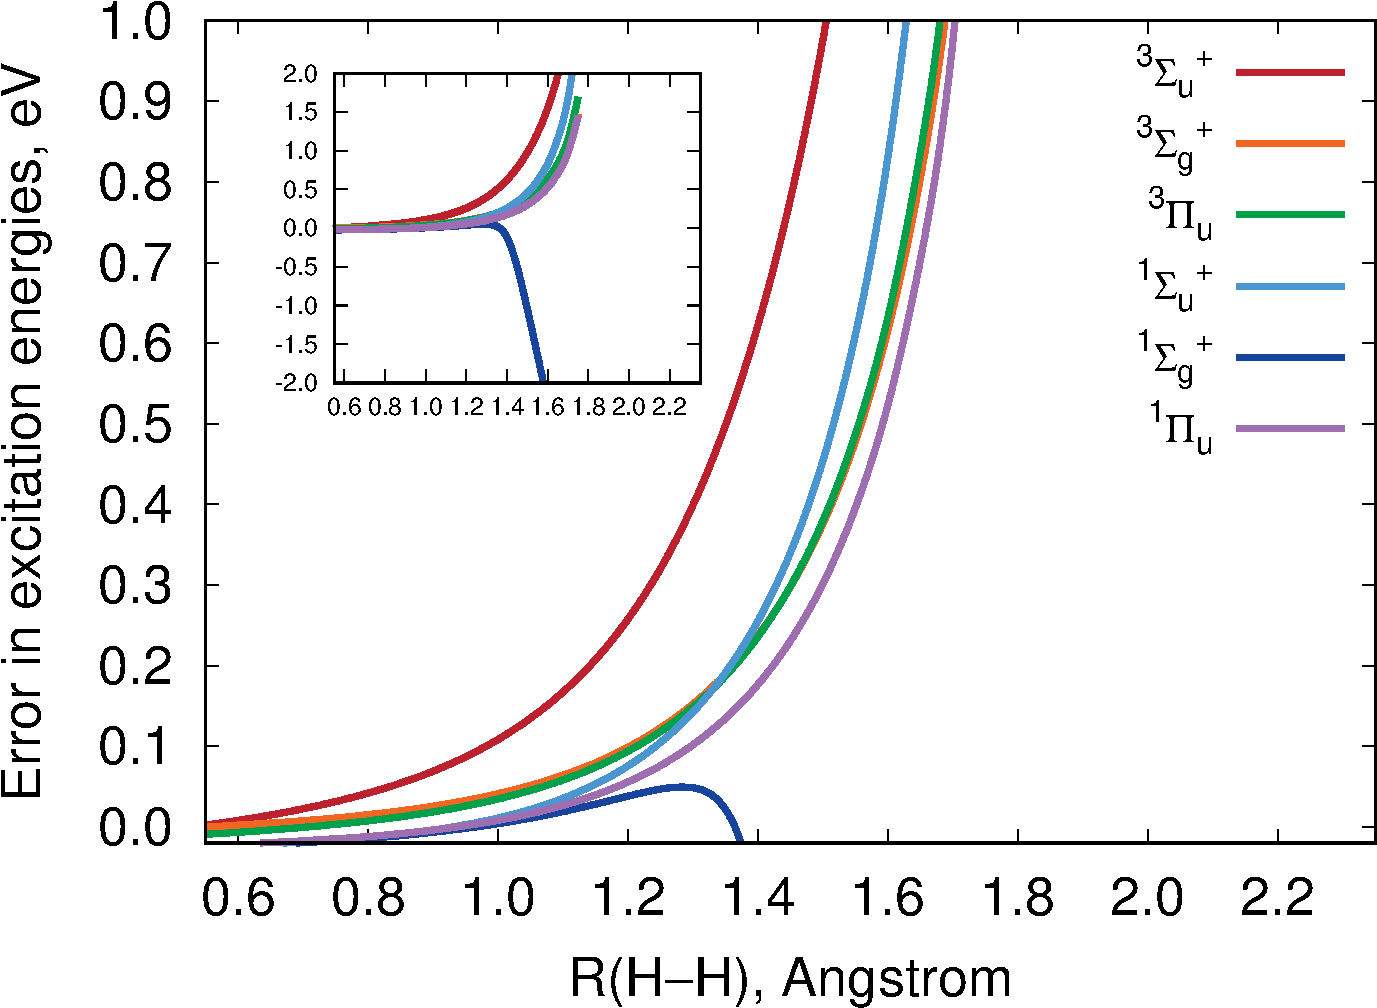
\includegraphics[width=0.45\textwidth]{figures/H2_olccd.pdf}} \quad
    \captionsetup{justification=raggedright,singlelinecheck=false}
    \caption{%
        \label{fig:H2_diss}
        Errors in vertical excitation energies (eV) for six lowest-lying
        electronic states of \ce{H2} computed using LR-ODC-12
        (\ref{fig:H2_diss_odc}) and LR-OLCCD (\ref{fig:H2_diss_olccd}) as a
        function of the H--H bond length, relative to full configuration
        interaction.
        All methods employed the d-aug-cc-pvtz basis set.
        In each figure, the inset shows the same plot for a larger range of
        errors.
    }
\end{figure*}

One of the desirable properties of an electronic structure method is exactness
for two-electron systems. While the ODC-12 method is not exact for two-electron
systems, it has been shown to provide a very good description of the
ground-state \ce{H2} dissociation curve, with errors of $\sim$ 1 \kcal with
respect to full configuration interaction (FCI) near the dissociation
limit.\cite{Sokolov:2013p204110} Here, we investigate the performance of
LR-ODC-12 for the excited states of \ce{H2}. \cref{fig:H2_diss_odc} shows the
errors in vertical excitation energies for six lowest-lying electronic states as
a function of the \ce{H-H} distance, relative to FCI\@. The FCI energies were
computed using the EOM-CCSD method, which is exact for two-electron systems. At
the equilibrium geometry (\re = 0.742 \AA) the errors in excitation energies
for all states do not exceed 0.02 eV. Between 0.6 and 1.45 \AA\
(\mbox{$r\approx2\re$}), the LR-ODC-12 excitation energies remain to be in a
good agreement with FCI, with errors less than 0.1 eV for all states. In this
range, the largest error is observed for the $^3\Sigma_u^+$ state. For $r$ $\ge$
1.5 \AA, the error in the $^1\Sigma_g^+$ excited state energy rapidly increases
from 0.10 eV (at 1.5 \AA) to 2.13 eV (at 2.35 \AA), while for other states the
errors increase much more slowly. Analysis of the FCI wavefunction for the
$^1\Sigma_g^+$ state shows a significant contribution from the
$(1\sigma_g)^2\rightarrow(1\sigma_u)^2$ double excitation already at $r$ $=$
1.55 \AA\@. This contribution becomes dominant for $r$ $\ge$ 1.75 \AA\@.
Thus, the large LR-ODC-12 errors observed for the $^1\Sigma_g^+$ state are
likely due to the double-excitation character of this electronic state at long
\ce{H-H} bond distances.
The second largest error near the dissociation is observed for the
$^3\Sigma_u^+$ state (0.43 eV).
For other electronic states, smaller errors of $\sim$ 0.25 eV are observed near
the dissociation.

We now compare the performance of LR-ODC-12 to that of the LR-OLCCD method,
which can be considered as an approximation to LR-ODC-12 where all of the
non-linear terms are removed in the description of electron correlation.
\Cref{fig:H2_diss_olccd} shows the errors in the LR-OLCCD vertical excitation
energies as a function of the \ce{H-H} bond length.
Although near the equilibrium geometry the performance of LR-OLCCD and LR-ODC-12
is similar, the LR-OLCCD errors increase much faster with increasing \ce{H-H}
distance compared to LR-ODC-12.
At $r$ = 1.3 \AA, the LR-OLCCD error for the $^3\Sigma_u^+$ state (0.4 eV) is
almost six times larger than the corresponding error from LR-ODC-12 (0.07 eV).
For $r$ $\ge$ 1.35 \AA, the LR-OLCCD errors for all excitation energies show
very steep increase in magnitude, ranging from 1.5 to 4.7 eV already at $r$ =
1.75 \AA\@. We were unable to converge the LR-OLCCD equations for $r$ $\ge$ 1.80
\AA\@.
Overall, our results demonstrate that the non-linear terms in LR-ODC-12
significantly improve the description of excited states at long \ce{H-H}
distances when the electron correlation effects become particularly strong.


\subsection{Benchmark: Small Molecules}
\label{sec:vert_excit}

\afterpage{%
    \clearpage
    \centering
    \vspace*{\fill}
    \captionof{table}{%
        \label{tab:vertical_singlet}
        Errors in vertical excitation energies (eV) for singlet states
        computed using LR-OLCCD, LR-ODC-12, and EOM-CCSD, relative to
        EOM-CCSDT (aug-cc-pVTZ basis set).
        All electrons were correlated in all computations.
        Also shown are mean absolute errors (\mae) and standard deviations
        (\std) computed for each method.
    }
    \begin{threeparttable}
        \small
        \renewcommand\arraystretch{0.6}
        \begin{tabular}{clcccc}
            \hline
            \hline
            &&
            \(\Delta\)EOM-CCSD & \(\Delta\)LR-OLCCD & \(\Delta\)LR-ODC-12 & 
            EOM-CCSDT \\
            \hline
            \ce{N2}
            & \({}^1\Pi_g\)        &
            \( \)0.18 & \( \)0.08 & \( \)0.20 &  9.29 \\
            & \({}^1\Sigma_u^-\)   &
            \( \)0.23 & \( \)0.15 & \( \)0.09 &  9.84 \\
            & \({}^1\Delta_u\)     &
            \( \)0.26 & \( \)0.14 & \( \)0.10 & 10.26 \\
            \ce{CO}                            
            & \({}^1\Pi\)          &
            \( \)0.16 & \( \)0.09 & \( \)0.17 &  8.46 \\
            & \({}^1\Sigma^-\)     &
            \( \)0.19 & \(-\)0.10 & \(-\)0.01 &  9.89 \\
            & \({}^1\Delta\)       &
            \( \)0.19 & \(-\)0.22 & \(-\)0.05 & 10.03 \\
            \ce{HCN}                           
            & \({}^1\Sigma^-\)     &
            \( \)0.16 & \( \)0.05 & \( \)0.00 & 8.25 \\
            & \({}^1\Delta\)       &
            \( \)0.17 & \( \)0.04 & \( \)0.01 & 8.61 \\
            & \({}^1\Pi\)          &
            \( \)0.17 & \( \)0.05 & \( \)0.20 & 9.12 \\
            \ce{HNC}                           
            & \({}^1\Pi\)          &
            \( \)0.15 & \(-\)0.01 & \( \)0.10 & 8.13 \\
            & \({}^1\Sigma^+\)     &
            \( \)0.24 & \( \)0.05 & \( \)0.12 & 8.46 \\
            & \({}^1\Sigma^-\)     &
            \( \)0.15 & \(-\)0.09 & \( \)0.04 & 8.67 \\
            & \({}^1\Delta\)       &
            \( \)0.15 & \(-\)0.18 & \(-\)0.03 & 8.84 \\
            \ce{H2C2}                          
            & \({}^1\Sigma_u^-\)   &
            \( \)0.12 & \( \)0.06 & \( \)0.02 & 7.11 \\
            & \({}^1\Delta_u\)     &
            \( \)0.10 & \( \)0.07 & \( \)0.03 & 7.45 \\
            \ce{H2CO}                                                 
            & \({}^1\mathrm{A_2}\) &
            \( \)0.10 & \(-\)0.07 & \( \)0.02 & 3.95 \\
            \hline
            \mae & & 0.09 & 0.08 & 0.17 &  \\		
            \std & & 0.11 & 0.08 & 0.05 &  \\ 		
            \hline
            \hline
        \end{tabular}
    \end{threeparttable}
    \vspace*{\fill}
    \newpage
    \vspace*{\fill}
    \captionof{table}{%
        \label{tab:vertical_triplet}
        Errors in vertical excitation energies (eV) for triplet states
        computed using LR-OLCCD, LR-ODC-12, and EOM-CCSD, relative to
        EOM-CCSDT (aug-cc-pVTZ basis set).
        All electrons were correlated in all computations.
        Also shown are mean absolute errors (\mae) and standard deviations
        (\std) computed for each method.
    }
    \begin{threeparttable}
        \small
        \renewcommand\arraystretch{0.6}
        \begin{tabular}{clcccc}
            \hline
            \hline
            &&
            \(\Delta\)EOM-CCSD & \(\Delta\)LR-OLCCD & \(\Delta\)LR-ODC-12 &
            EOM-CCSDT\tnote{a} \\
            \hline
            \ce{N2}
            & \({}^3\Sigma_u^+\)   &
            \( \)0.11 & \( \)0.04 & \(-\)0.02 &  7.63 \\\
            & \({}^3\Pi_g\)        &
            \( \)0.15 & \( \)0.06 & \( \)0.11 &  8.00 \\\
            & \({}^3\Delta_u\)     &
            \( \)0.17 & \( \)0.08 & \( \)0.03 &  8.82 \\\
            & \({}^3\Sigma_u^-\)   &
            \( \)0.28 & \( \)0.03 & \( \)0.01 &  9.63 \\\
            & \({}^3\Pi_u\)        &
            \( \)0.14 & \(-\)0.01 & \( \)0.10 & 11.18 \\\
            \ce{CO}                            
            & \({}^3\Pi\)          &
            \( \)0.12 & \( \)0.06 & \( \)0.08 &  6.27 \\\
            & \({}^3\Sigma^+\)     &
            \( \)0.05 & \(-\)0.03 & \(-\)0.03 &  8.38 \\\
            & \({}^3\Delta\)       &
            \( \)0.11 & \(-\)0.07 & \(-\)0.03 &  9.21 \\\
            & \({}^3\Sigma^-\)     &
            \( \)0.19 & \(-\)0.18 & \(-\)0.06 &  9.72 \\\
            \ce{HCN}                           
            & \({}^3\Sigma^+\)     &
            \( \)0.05 & \(-\)0.04 & \(-\)0.10 &  6.40 \\
            & \({}^3\Delta\)       &
            \( \)0.13 & \(-\)0.02 & \(-\)0.06 &  7.40 \\
            & \({}^3\Pi\)          &
            \( \)0.10 & \( \)0.08 & \( \)0.06 &  8.01 \\
            & \({}^3\Sigma^-\)     &
            \( \)0.16 & \(-\)0.10 & \(-\)0.05 &  8.15 \\
            \ce{HNC}                                                      
            & \({}^3\Pi\)          &
            \( \)0.09 & \( \)0.00 & \( \)0.03 &  6.06 \\
            & \({}^3\Sigma^+\)     &
            \( \)0.04 & \(-\)0.09 & \(-\)0.11 &  7.20 \\
            & \({}^3\Delta\)       &
            \( \)0.10 & \(-\)0.14 & \(-\)0.11 &  8.02 \\
            & \({}^3\Sigma^+\)     &
            \( \)0.22 & \(-\)0.05 & \( \)0.04 &  8.38 \\
            & \({}^3\Sigma^-\)     &
            \( \)0.15 & \(-\)0.02 & \( \)0.11 &  8.56 \\
            \ce{H2C2}                                                     
            & \({}^3\Sigma_u^+\)   &
            \( \)0.01 & \(-\)0.02 & \(-\)0.08 &  5.52 \\
            & \({}^3\Delta_u\)     &
            \( \)0.08 & \(-\)0.02 & \(-\)0.05 &  6.41 \\
            & \({}^3\Sigma_u^-\)   &
            \( \)0.10 & \(-\)0.03 & \(-\)0.05 &  7.10 \\
            \ce{H2CO}                                                     
            & \({}^3\mathrm{A_2}\) &
            \( \)0.04 & \(-\)0.02 & \( \)0.01 &  3.56 \\
            & \({}^3\mathrm{A_1}\) &
            \( \)0.02 & \(-\)0.06 & \(-\)0.14 &  6.06 \\
            \hline
            \mae && 0.17 & 0.09 & 0.08 & \\		
            \std && 0.05 & 0.11 & 0.08 & \\ 		
            \hline
            \hline
        \end{tabular}
        \begin{tablenotes}
        \item[a]
            For CO, HCN, HNC, and \ce{H2C2}, the ${}^3\Sigma^-$
            (${}^3\Sigma_u^-$) excitation energies were obtained from
            EOM-CC(2,3), which energies were shifted to reproduce the
            EOM-CCSDT energy for the ${}^1\Sigma^-$ (${}^1\Sigma_u^-$)
            state.
        \end{tablenotes}    
    \end{threeparttable}
    \vspace*{\fill}
    \newpage
    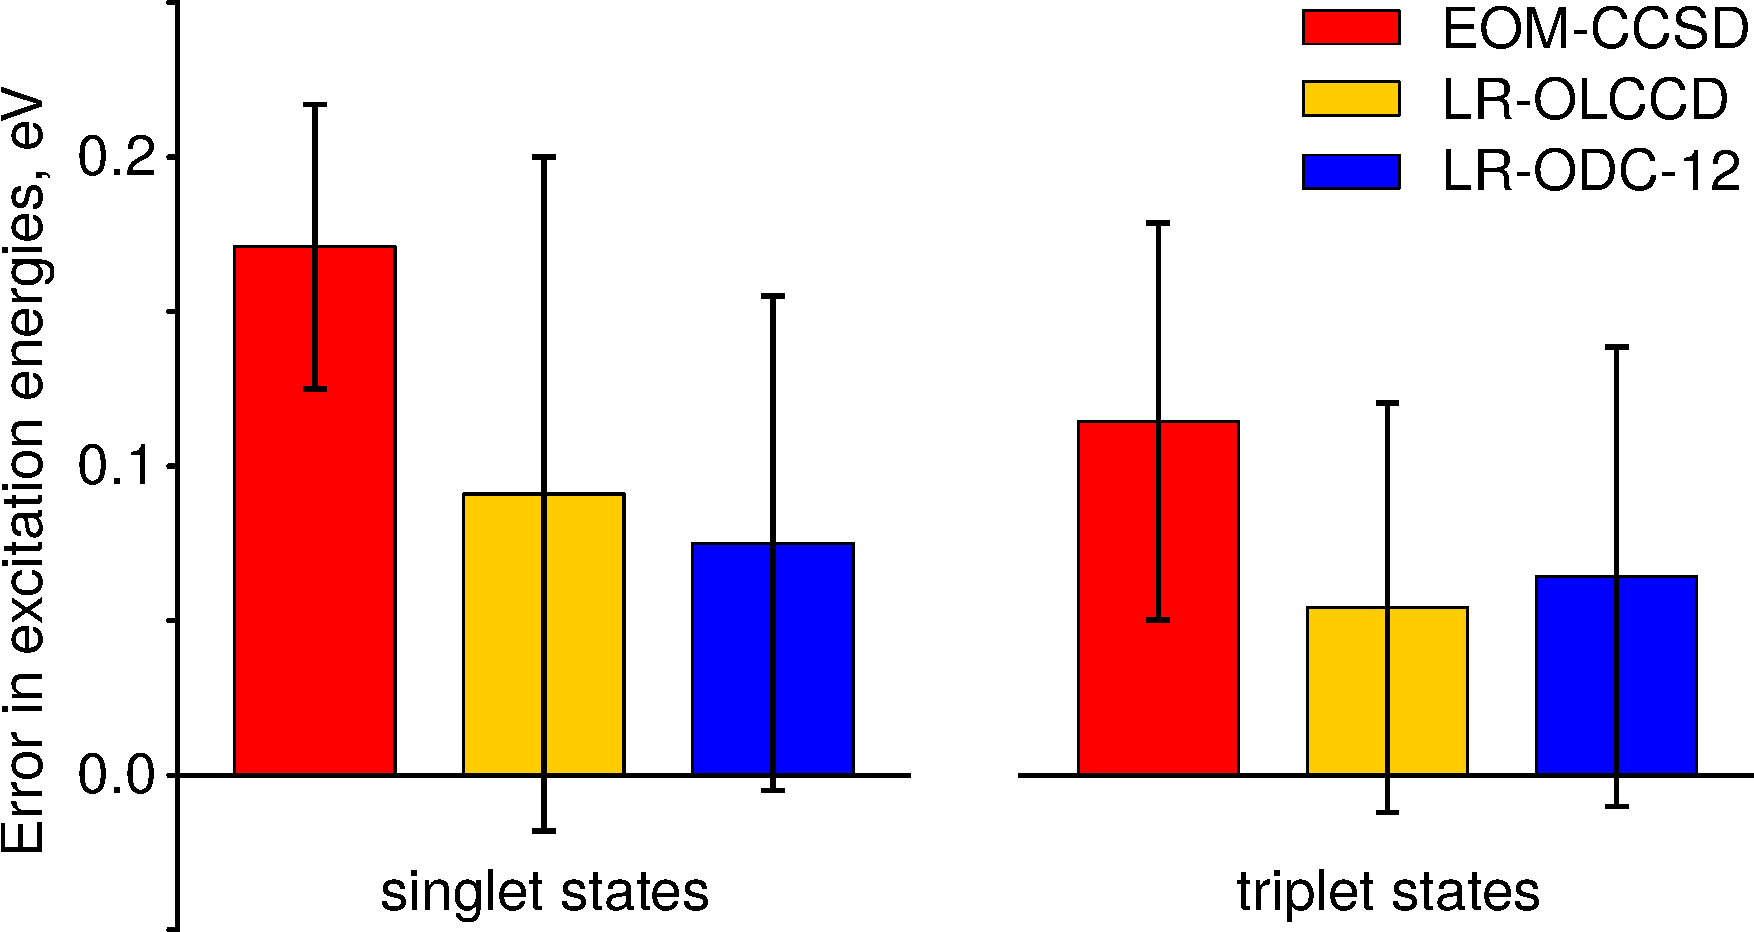
\includegraphics[width=0.8\textwidth]{figures/excitation-energies.pdf}
    \captionof{figure}{%
        \label{fig:vertical_mae}
        Mean absolute deviations (\mae) and standard deviations from the
        mean signed error (\std) in vertical excitation energies for the
        states in \cref{tab:vertical_singlet,tab:vertical_triplet} for
        OLCCD, LR-ODC-12, and EOM-CCSD relative to EOM-CCSDT (aug-cc-pVTZ
        basis set).
        The height of each colored box represents the \mae value of the
        method and the height of the black bar above each box represents its
        \std value.
    }
}


Here we investigate the performance of our method for vertical excitation
energies in several small molecules: \ce{N2}, \ce{CO}, \ce{HCN}, \ce{HNC},
\ce{H2C2}, and \ce{H2CO}.
The reference values have been computed with EOM-CCSDT and we compare
all-electron calculations with the same aug-cc-pVTZ basis in order to exclude
basis set incompleteness error from the comparison.
As an aggregate measure of the tendency for each method to deviate from the
reference values, we calculate their mean absolute errors (\mae).
As a measure of the degree to which the errors are systematically clustered
above or below the reference values, we look at their standard deviation from
the average signed error (\std).

For the singlets, LR-ODC-12 has errors above 0.15~eV for three states, with a
maximum error of 0.20~eV.
All three of these occur for \({}^1\Pi\) states of linear molecules, which are
dominated by \(\sigma\rightarrow\pi^*\) excitations.
EOM-CCSD has eleven errors greater than 0.15~eV, with a maximum error of 0.26~eV
and no predictable pattern -- the largest three errors occur for three
qualitatively unrelated states: \({}^1\Delta\), \({}^1\Sigma^-\), and
\({}^1\Sigma^+\).
Interestingly, the EOM-CCSD errors are relatively tightly clustered around their
mean error of 0.17~eV, with a standard deviation of 0.05~eV compared to 0.08~eV
for LR-OCD-12.
For the triplets, LR-ODC-12 has no errors at all above 0.15~eV, whereas EOM-CCSD
has six, with a maximum error of 0.28~eV for the \({}^3\Sigma_u^-\) state of
\ce{N2}.
Here the EOM-CCSD description of \({}^3\Sigma^-\) states is consistently poor,
but some of the larger errors occur for \({}^3\Sigma^+\) and \({}^3\Delta\)
states as well.
In aggregate, we see that LR-ODC-12 cuts the mean absolute errors of EOM-CCSD
roughly in half for both singlet and triplet states.
Notably, whereas the EOM-CCSD errors are exclusively positive, the LR-ODC-12
errors are more centered on 0~eV, suggesting a more balanced treatment of the
ground and excited states.

Comparing LR-ODC-12 to LR-OLCCD we see that most of the errors are within 0.1~eV
of each other, suggesting that the non-linear terms are relatively unimportant
for many of these states.
Significant differences occur for the \({}^1\Delta\) states of CO and HCN, where
LR-OLCCD shows some deterioration, and for the \({}^1\Pi\) state of HCN,
where the linearization leads to a significant error cancellation.


% \section{Conclusions}
% \label{sec:conclusions}
% 
% Our conclusions.

\begin{subappendices}
    \section{%
        Derivatives of the One-Body Density Matrix in Density Cumulant Theory
    }
    \label{sec:appendix}

    Repeated differentiation of the one-body \(n\)-representability condition in
    DCT (\cref{eq:one-body-n-rep}) gives the following formulas for the first
    and second derivatives of the cumulant partial trace:
    \begin{equation}
        \begin{array}{r@{\,}l}
            \dfrac{\partial \lambda^{pr}_{qr}}{\partial{y}}
            =
            \gamma^p_s
            \dfrac{\partial \gamma^s_q}{\partial{y}}
            +
            \dfrac{\partial \gamma^p_s}{\partial{y}}
            \gamma^s_q
            -
            \dfrac{\partial \gamma^p_q}{\partial{y}}
        \end{array}
    \end{equation}
    \begin{equation}
        \begin{array}{r@{\,}l}
            \dfrac{\partial^2 \lambda^{pr}_{qr}}{%
                \partial{x}
                \partial{y}
            }
            =
            &
            \gamma^p_s
            \dfrac{\partial \gamma^s_q}{%
                \partial{x}
                \partial{y}
            }
            +
            \dfrac{\partial \gamma^p_s}{%
                \partial{x} \partial{y}
            }
            \gamma^s_q
            -
            \dfrac{\partial \gamma^p_q}{%
                \partial{x}
                \partial{y}
            }
            \\[15pt]
            &
            +
            \dfrac{\partial \gamma^p_s}{\partial{x}}
            \dfrac{\partial \gamma^s_q}{\partial{y}}
            +
            \dfrac{\partial \gamma^s_q}{\partial{x}}
            \dfrac{\partial \gamma^p_s}{\partial{y}}
        \end{array}
    \end{equation}
    Transforming to the natural spin-orbital basis (NSO, denoted by prime
    indices) where the one-body density matrix is diagonal, the first and second
    derivatives of the one-body density matrix can be determined from the
    cumulant derivatives as follows:
    \begin{equation}
        \label{eq:one-body-n-rep-gradient}
        \begin{array}{r@{\,}l}
            \dfrac{\partial \gamma^{p'}_{q'}}{\partial{y}}
            =
            &
            \theta_{p'q'}
            \dfrac{\partial \lambda^{p'r}_{q'r}}{\partial{y}}
        \end{array}
    \end{equation}
    \begin{equation}
        \label{eq:one-body-n-rep-hessian}
        \begin{array}{r@{\,}l}
            \dfrac{\partial^2 \gamma^{p'}_{q'}}{%
                \partial{x}
                \partial{y}
            }
            =
            &
            \theta_{p'q'}
            \dfrac{\partial^2 \lambda^{p'r}_{q'r}}{%
                \partial{x}
                \partial{y}
            }
            -
            \delta_{r'}^{s'}
            \theta_{p'q'}
            \theta_{p's'}
            \theta_{q'r'}
            \dfrac{\partial \lambda^{p't}_{s't}}{%
                \partial{x}
            }
            \dfrac{\partial \lambda^{r'u}_{q'u}}{\partial{y}}
            \\[15pt]
            &
            -
            \delta_{r'}^{s'}
            \theta_{p'q'}
            \theta_{p's'}
            \theta_{q'r'}
            \dfrac{\partial \lambda^{r'u}_{q'u}}{\partial{x}}
            \dfrac{\partial \lambda^{p't}_{s't}}{\partial{y}}
        \end{array}
    \end{equation}
    Here, we have defined the following matrix:
    \begin{equation}
        \theta_{p'q'}
        \equiv
        \left\{
            \begin{array}{cc}
                (
                    \gamma_{p'}
                    +
                    \gamma_{q'}
                    -
                    1
                )^{-1}
                &
                \text{%
                    if
                    \(p',q'\in \mathrm{occ \ or \ vir}\)
                }
                \\
                0
                &
                \text{otherwise}
            \end{array}
        \right.
    \end{equation}
    where \(\gamma_{p'}\) denotes an eigenvalue of the one-body density matrix
    (i.e., an occupation number).
    The natural spin-orbital $p'$ is occupied if \(\gamma_{p'} > 0.5\).

    \Cref{eq:one-body-n-rep-gradient,eq:one-body-n-rep-hessian} can be used to
    derive expression for the two-body energy Hessian in
    \cref{eq:odc12-hessian-initial-form}.
    Simplifying the resulting equations allows us to determine the intermediates
    defined in \cref{eq:a22_odc12}.
    In the NSO basis, these intermediates are given by
    \begin{equation}
        \label{eq:fancy-f-intermediate}
        \mathcal{F}_{p'}^{q'}
        \equiv
        \theta_{p'q'}
        f_{p'}^{q'}
    \end{equation}
    \begin{equation}
        \label{eq:fancy-g-intermediate}
        \mathcal{G}_{p'r'}^{q's'}
        \equiv
        \theta_{p'q'}
        \theta_{r's'}
        (
            \overline{g}_{p'r'}^{q's'}
            -
            \mathcal{F}_{p'}^{s'}
            \delta_{r'}^{q'}
            -
            \mathcal{F}_{r'}^{q'}
            \delta_{p'}^{s'}
        )
    \end{equation}
    Although these intermediates are computed in the NSO basis, they must be
    back-transformed to the original spin-orbital basis using the eigenvectors
    of the one-particle density matrix before being used in \cref{eq:a22_odc12}
    (see Ref.\@ \citenum{Sokolov:2013p024107} for more details).


    \section{Supporting Information}
    \label{sec:suppinfo}

    Here, we present the working equations for the LR-ODC-12 and LR-OLCCD
    methods.
    We refer the reader to the main article for definitions and notation, and
    note that prime indices refer to the natural spin-orbital basis (NSO) where
    the one-particle density matrix is diagonal,
    \(\gamma^{p'}_{q'}=\delta^{p'}_{q'}\gamma_{q'}\).
    Quantities computed in the NSO basis can be back-transformed to the original
    basis using the eigenvectors of the one-particle density matrix.

    For the property gradient vectors, we define the block structure as follows
    \begin{equation}
        \mathbf{v}'^\dagger
        \equiv
        (\mathbf{p}_1\ \mathbf{p}_2\ \mathbf{p}_1^*\ \mathbf{p}_2^*)^\dagger
        \qquad
        \mathbf{p}_m
        \equiv
        \frac{%
            \partial \langle\Psi|\hat{V}|\Psi\rangle
        }{%
            \partial \mathbf{t}_m^\dagger
        }
    \end{equation}
    where \(\hat{V}\) can be any one-particle operator, defined through its
    spin-orbital integrals, \(v_p^q=\langle\psi_p|\hat{v}|\psi_q\rangle\), as
    follows.
    \begin{equation}
        \hat{V}
        =
        v_p^q
        a^p_q
    \end{equation}
    A typical example would be an electric dipole operator.

    \subsection{Working Equations for LR-ODC-12}

    \subsubsection{Density Matrices}

    \begin{equation}
        \gamma^i_j
        =
        \tfrac{1}{2}
        (
            \mathbf{1}
            +
            \sqrt{\mathbf{1} + 4\mathbf{d}}
        )_j^i
        \qquad
        (\mathbf{d})_j^i
        \equiv
        -
        \tfrac{1}{2}
        t_{cd}^{ik}
        t_{jk}^{cd*}
    \end{equation}

    \begin{equation}
        \gamma^b_a
        =
        \tfrac{1}{2}
        (
            \mathbf{1}
            -
            \sqrt{\mathbf{1} + 4\mathbf{d}}
        )_a^b
        \qquad
        (\mathbf{d})_a^b
        \equiv
        -
        \tfrac{1}{2}
        t_{ac}^{kl}
        t_{kl}^{bc*}
    \end{equation}

    \begin{equation}
        \gamma^{ij}_{kl}
        =
        \tfrac{1}{2}
        t_{cd}^{ij}
        t_{kl}^{cd*}
        +
        P_{(k/l)}
        \gamma^i_k
        \gamma^j_l
    \end{equation}

    \begin{equation}
        \gamma_{ab}^{cd}
        =
        \tfrac{1}{2}
        t_{ab}^{kl}
        t_{kl}^{cd*}
        +
        P^{(c/d)}
        \gamma_a^c
        \gamma_b^d
    \end{equation}

    \begin{equation}
        \gamma_{ja}^{ib}
        =
        -
        t_{ac}^{ik}
        t_{jk}^{bc*}
        +
        \gamma^i_j
        \gamma_a^b
    \end{equation}

    \begin{equation}
        \gamma_{ab}^{ij}
        =
        t_{ab}^{ij}
    \end{equation}


    \subsubsection{Blocks of the Energy Hessian}

    \begin{equation}
        \label{eq:a11-odc12-formula}
        \begin{array}{r@{\,}l}
            (\mathbf{A}_{11})_{ia,jb}
            =
            &
            h_j^i
            \gamma_a^b
            +
            h_a^b
            \gamma_j^i
            -
            (\bar{\mathbf{F}})_j^i
            \delta_a^b
            -
            (\bar{\mathbf{F}})_a^b
            \delta_j^i
            +
            \overline{g}_{nj}^{mi}
            \gamma_{ma}^{nb}
            +
            \overline{g}_{ma}^{nb}
            \gamma_{nj}^{mi}
            +
            \overline{g}_{jf}^{ie}
            \gamma_{ae}^{bf}
            +
            \overline{g}_{ae}^{bf}
            \gamma_{jf}^{ie}
            \\[5pt]
            &
            +
            \overline{g}_{me}^{ib}
            \gamma_{ja}^{me}
            +
            \overline{g}_{ja}^{me}
            \gamma_{me}^{ib}
        \end{array}
    \end{equation}

    \begin{equation}
        \bar{\mathbf{F}}
        \equiv
        \tfrac{1}{2}
        (\mathbf{F} + \mathbf{F}^\dagger)
        \qquad
        (\mathbf{F})_p^q
        \equiv
        h_p^t
        \gamma_t^q
        +
        \tfrac{1}{2}
        \overline{g}_{pt}^{uv}
        \gamma_{uv}^{qt}
    \end{equation}

    \begin{equation}
        \label{eq:b11-odc12-formula}
        \begin{array}{r@{\,}l}
            (\mathbf{B}_{11})_{ia,jb}
            =
            &
            \overline{g}_{be}^{im}
            \gamma_{ma}^{je}
            +
            \overline{g}_{ma}^{je}
            \gamma_{be}^{im}
            +
            \overline{g}_{mb}^{ie}
            \gamma_{ae}^{jm}
            +
            \overline{g}_{ae}^{jm}
            \gamma_{mb}^{ie}
            +
            \tfrac{1}{2}
            \overline{g}_{mn}^{ij}
            \gamma_{ab}^{mn}
            +
            \tfrac{1}{2}
            \overline{g}_{ab}^{mn}
            \gamma_{mn}^{ij}
            \\[5pt]
            &
            +
            \tfrac{1}{2}
            \overline{g}_{ef}^{ij}
            \gamma_{ab}^{ef}
            +
            \tfrac{1}{2}
            \overline{g}_{ab}^{ef}
            \gamma_{ef}^{ij}
        \end{array}
    \end{equation}

    \begin{equation}
        \label{eq:a22-odc12-formula}
        \begin{array}{r@{\,}l}
            (\mathbf{A}_{22})_{ijab,klcd}
            =
            &
            -
            P_{(a/b|k/l)}^{(c/d)}
            \mathcal{F}_a^c
            \delta_b^d
            \delta_k^i
            \delta_l^j
            -
            P_{(k/l)}^{(i/j|c/d)}
            \mathcal{F}_k^i
            \delta_l^j
            \delta_a^c
            \delta_b^d
            +
            P_{(k/l)}
            \overline{g}_{ab}^{cd}
            \delta_k^i
            \delta_l^j
            +
            P^{(c/d)}
            \overline{g}_{kl}^{ij}
            \delta_a^c
            \delta_b^d
            \\[5pt]
            &
            -
            P_{(a/b|k/l)}^{(i/j|c/d)}
            \overline{g}_{la}^{jc}
            \delta_b^d
            \delta_k^i
            +
            P_{(a/b)}^{(c/d)}
            \mathcal{G}_{af}^{ec}
            t_{eb}^{ij}
            t_{kl}^{fd*}
            +
            P_{(a/b|k/l)}
            \mathcal{G}_{ka}^{me}
            t_{eb}^{ij}
            t_{ml}^{cd*}
            \\[5pt]
            &
            +
            P^{(i/j|c/d)}
            \mathcal{G}_{me}^{ic}
            t_{ab}^{mj}
            t_{kl}^{ed*}
            +
            P_{(k/l)}^{(i/j)}
            \mathcal{G}_{mk}^{in}
            t_{ab}^{mj}
            t_{nl}^{cd*}
        \end{array}
    \end{equation}

    \begin{equation}
        \mathcal{F}_{p'}^{q'}
        \equiv
        \theta_{p'q'}
        f_{p'}^{q'}
        \qquad
        \mathcal{G}_{p'r'}^{q's'}
        \equiv
        \theta_{p'q'}
        \theta_{r's'}
        (
            \overline{g}_{p'r'}^{q's'}
            -
            \mathcal{F}_{p'}^{s'}
            \delta_{r'}^{q'}
            -
            \mathcal{F}_{r'}^{q'}
            \delta_{p'}^{s'}
        )
    \end{equation}

    \begin{equation}
        \theta_{p'q'}
        \equiv
        \left\{
            \begin{array}{cc}
                (
                    \gamma_{p'}
                    +
                    \gamma_{q'}
                    -
                    1
                )^{-1}
                &
                \text{%
                    if
                    \(p,q\in \mathrm{occ \ or \ vir}\)
                }
                \\
                0
                &
                \text{otherwise}
            \end{array}
        \right.
    \end{equation}

    \begin{equation}
        \begin{array}{r@{\,}l}
            (\mathbf{B}_{22})_{ijab,klcd}
            =
            &
            P_{(a/b|c/d)}
            \mathcal{G}_{ac}^{ef}
            t_{eb}^{ij}
            t_{fd}^{kl}
            +
            P_{(a/b)}^{(k/l)}
            \mathcal{G}_{na}^{ke}
            t_{eb}^{ij}
            t_{cd}^{nl}
            +
            P_{(c/d)}^{(i/j)}
            \mathcal{G}_{mc}^{if}
            t_{ab}^{mj}
            t_{fd}^{kl}
            \\[5pt]
            &
            +
            P^{(i/j|k/l)}
            \mathcal{G}_{mn}^{ik}
            t_{ab}^{mj}
            t_{cd}^{nl}
        \end{array}
    \end{equation}

    \begin{equation}
        \begin{array}{r@{\,}l}
            (\mathbf{A}_{12})_{ia,klcd}
            =
            &
            P_{(k/l)}
            \overline{g}_{la}^{cd}
            \delta_k^i
            +
            P^{(c/d)}
            \overline{g}_{kl}^{id}
            \delta_a^c
            +
            P_{(k/l)}
            (\mathcal{I}_a^i)_k^m
            t_{ml}^{cd*}
            +
            P^{(c/d)}
            (\mathcal{I}_a^i)_e^c
            t_{kl}^{ed*}
            \\[5pt]
            &
            +
            P_{(k/l)}^{(c/d)}
            \overline{g}_{ae}^{mc}
            t_{ml}^{ed*}
            \delta_k^i
            +
            P_{(k/l)}^{(c/d)}
            \overline{g}_{ke}^{im}
            t_{ml}^{ed*}
            \delta_a^c
            +
            \tfrac{1}{2}
            P_{(k/l)}
            \overline{g}_{la}^{mn}
            t_{mn}^{cd*}
            \delta_k^i
            \\[5pt]
            &
            +
            \tfrac{1}{2}
            P^{(c/d)}
            \overline{g}_{ef}^{id}
            t_{kl}^{ef*}
            \delta_a^c
        \end{array}
    \end{equation}

    \begin{equation}
        \begin{array}{r@{\,}l}
            (\mathbf{B}_{12})_{ia,klcd}
            =
            &
            P^{(k/l)}
            (\mathcal{I}_a^i)_m^k
            t_{cd}^{ml}
            +
            P_{(c/d)}
            (\mathcal{I}_a^i)_c^e
            t_{ed}^{kl}
            +
            P_{(c/d)}^{(k/l)}
            \overline{g}_{ad}^{le}
            t_{ce}^{ki}
            +
            P_{(c/d)}^{(k/l)}
            \overline{g}_{md}^{il}
            t_{ca}^{km}
            +
            \overline{g}_{ma}^{kl}
            t_{cd}^{im}
            \\[5pt]
            &
            +
            \overline{g}_{cd}^{ie}
            t_{ae}^{kl}
        \end{array}
    \end{equation}

    \begin{equation}
        (\mathcal{I}_a^i)_{k'}^{l'}
        \equiv
        \theta_{k'l'}
        (I_a^i)_{k'}^{l'}
        \qquad
        (I_a^i)_k^l
        \equiv
        +
        f_a^l
        \delta_k^i
        -
        \overline{g}_{ka}^{ml}
        \gamma_m^i
        +
        \overline{g}_{ke}^{il}
        \gamma_a^e
    \end{equation}

    \begin{equation}
        (\mathcal{I}_a^i)_{c'}^{d'}
        \equiv
        \theta_{c'd'}
        (I_a^i)_{c'}^{d'}
        \qquad
        (I_a^i)_c^d
        \equiv
        -
        f_c^i
        \delta_a^d
        +
        \overline{g}_{ac}^{md}
        \gamma_m^i
        -
        \overline{g}_{ec}^{id}
        \gamma_a^e
    \end{equation}

    \subsubsection{Blocks of the Metric Matrix}

    \begin{equation}
        \label{eq:s11-odc12}
        \begin{array}{r@{\,}l}
            (\mathbf{S}_{11})_{ia,jb}
            &=
            (
                \delta^b_a
                \gamma^i_j
                -
                \delta^i_j
                \gamma^b_a
            )
        \end{array}
    \end{equation}

    \subsubsection{Blocks of the Property Gradient Vector}

    \begin{equation}
        \label{eq:p1-odc12}
        (\mathbf{p}_1)_{ia}
        =
        v_a^k
        \gamma_k^i
        -
        v_c^i
        \gamma_a^c
    \end{equation}

    \begin{equation}
        (\mathbf{p}_2)_{ijab}
        =
        -
        P_{(a/b)}
        \mathcal{V}_a^e
        t_{eb}^{ij}
        -
        P^{(i/j)}
        \mathcal{V}_m^i
        t_{ab}^{mj}
    \end{equation}

    \begin{equation}
        \mathcal{V}_{p'}^{q'}
        \equiv
        \theta_{p'q'}
        v_{p'}^{q'}
    \end{equation}

    \subsection{Working Equations for LR-OLCCD}

    \subsubsection{Density Matrices}

    \begin{equation}
        \gamma^i_j
        =
        \delta^i_j
        -
        \tfrac{1}{2}
        t_{cd}^{ik}
        t_{jk}^{cd*}
    \end{equation}

    \begin{equation}
        \gamma^b_a
        =
        \tfrac{1}{2}
        t_{ac}^{kl}
        t_{kl}^{bc*}
    \end{equation}

    \begin{equation}
        \gamma^{ij}_{kl}
        =
        \tfrac{1}{2}
        t_{cd}^{ij}
        t_{kl}^{cd*}
        +
        P_{(k/l)}
        \delta^i_k
        \delta^j_l
        +
        \tfrac{1}{2}
        P_{(k/l)}^{(i/j)}
        \delta^i_k
        t_{cd}^{jm}
        t_{lm}^{cd*}
    \end{equation}

    \begin{equation}
        \gamma_{ab}^{cd}
        =
        \tfrac{1}{2}
        t_{ab}^{kl}
        t_{kl}^{cd*}
    \end{equation}

    \begin{equation}
        \gamma_{ja}^{ib}
        =
        -
        t_{ac}^{ik}
        t_{jk}^{bc*}
        +
        \tfrac{1}{2}
        \delta^i_j
        t_{ac}^{kl}
        t_{kl}^{bc*}
    \end{equation}

    \begin{equation}
        \gamma_{ab}^{ij}
        =
        t_{ab}^{ij}
    \end{equation}

    \subsubsection{Blocks of the Energy Hessian}

    \begin{equation}
        (\mathbf{A}_{11})_{ia,jb}
        =
        \text{%
            \Cref{eq:a11-odc12-formula} with OLCCD density matrices.
        }
    \end{equation}

    \begin{equation}
        (\mathbf{B}_{11})_{ia,jb}
        =
        \text{%
            \Cref{eq:b11-odc12-formula} with OLCCD density matrices.
        }
    \end{equation}

    \begin{equation}
        \begin{array}{r@{\,}l}
            (\mathbf{A}_{22})_{ijab,klcd}
            =
            &
            P_{(a/b|k/l)}^{(c/d)}
            (\mathbf{f}_0)_a^c
            \delta_b^d
            \delta_k^i
            \delta_l^j
            -
            P_{(k/l)}^{(i/j|c/d)}
            (\mathbf{f}_0)_k^i
            \delta_l^j
            \delta_a^c
            \delta_b^d
            +
            P_{(k/l)}
            \overline{g}_{ab}^{cd}
            \delta_k^i
            \delta_l^j
            \\[5pt]
            &
            +
            P^{(c/d)}
            \overline{g}_{kl}^{ij}
            \delta_a^c
            \delta_b^d
            -
            P_{(a/b|k/l)}^{(i/j|c/d)}
            \overline{g}_{la}^{jc}
            \delta_b^d
            \delta_k^i
        \end{array}
    \end{equation}

    \begin{equation}
        (\mathbf{f}_0)_p^q
        =
        h_p^q
        +
        \overline{g}_{pi}^{qi}
    \end{equation}

    \begin{equation}
        \begin{array}{r@{\,}l}
            (\mathbf{B}_{22})_{ijab,klcd}
            =
            0
        \end{array}
    \end{equation}

    \begin{equation}
        \begin{array}{r@{\,}l}
            (\mathbf{A}_{12})_{ia,klcd}
            =
            &
            P_{(k/l)}
            \overline{g}_{la}^{cd}
            \delta_k^i
            +
            P^{(c/d)}
            \overline{g}_{kl}^{id}
            \delta_a^c
            +
            P_{(k/l)}
            (I_a^i)_k^m
            t_{ml}^{cd*}
            -
            P^{(c/d)}
            (I_a^i)_e^c
            t_{kl}^{ed*}
            \\[5pt]
            &
            +
            P_{(k/l)}^{(c/d)}
            \overline{g}_{ae}^{mc}
            t_{ml}^{ed*}
            \delta_k^i
            +
            P_{(k/l)}^{(c/d)}
            \overline{g}_{ke}^{im}
            t_{ml}^{ed*}
            \delta_a^c
            +
            \tfrac{1}{2}
            P_{(k/l)}
            \overline{g}_{la}^{mn}
            t_{mn}^{cd*}
            \delta_k^i
            \\[5pt]
            &
            +
            \tfrac{1}{2}
            P^{(c/d)}
            \overline{g}_{ef}^{id}
            t_{kl}^{ef*}
            \delta_a^c
        \end{array}
    \end{equation}

    \begin{equation}
        (I_a^i)_k^l
        \equiv
        +
        f_a^l
        \delta_k^i
        -
        \overline{g}_{ka}^{il}
        \qquad
        (I_a^i)_c^d
        \equiv
        -
        f_c^i
        \delta_a^d
        +
        \overline{g}_{ac}^{id}
    \end{equation}

    \begin{equation}
        \begin{array}{r@{\,}l}
            (\mathbf{B}_{12})_{ia,klcd}
            =
            &
            P^{(k/l)}
            (I_a^i)_m^k
            t_{cd}^{ml}
            -
            P_{(c/d)}
            (I_a^i)_c^e
            t_{ed}^{kl}
            +
            P_{(c/d)}^{(k/l)}
            \overline{g}_{ad}^{le}
            t_{ce}^{ki}
            +
            P_{(c/d)}^{(k/l)}
            \overline{g}_{md}^{il}
            t_{ca}^{km}
            +
            \overline{g}_{ma}^{kl}
            t_{cd}^{im}
            \\[5pt]
            &
            +
            \overline{g}_{cd}^{ie}
            t_{ae}^{kl}
        \end{array}
    \end{equation}

    \subsubsection{Blocks of the Metric Matrix}

    \begin{equation}
        (\mathbf{S}_{11})_{ia,jb}
        =
        \text{%
            \Cref{eq:s11-odc12} with OLCCD density matrices.
        }
    \end{equation}

    \subsubsection{Blocks of the Property Gradient Vector}

    \begin{equation}
        (\mathbf{p}_1)_{ia}
        =
        \text{%
            \Cref{eq:p1-odc12} with OLCCD density matrices.
        }
    \end{equation}

    \begin{equation}
        (\mathbf{p}_2)_{ijab}
        =
        P_{(a/b)}
        v_a^e
        t_{eb}^{ij}
        -
        P^{(i/j)}
        v_m^i
        t_{ab}^{mj}
    \end{equation}

\end{subappendices}
